\documentclass{beamer}
\usetheme[deutsch]{KIT}

\usepackage[utf8]{inputenc}
\usepackage[T1]{fontenc}
\usepackage{babel}
\usepackage{tikz,calc,ifthen}
\usepackage{mathtools}
\usepackage[normalem]{ulem}
\usepackage{graphicx}
\usepackage{listings}

\usepackage{xcolor}
\definecolor{darkblue}{RGB}{0,0,200}
\definecolor{darkred}{RGB}{200,0,0}
\definecolor{darkgreen}{RGB}{0,160,0}
\definecolor{darkbrown}{RGB}{160,30,70}
\definecolor{darkorange}{RGB}{255, 102, 0}
\definecolor{darkturqoise}{RGB}{0,170,136}
\definecolor{darkdarkblue}{RGB}{212,0,170}

\usetikzlibrary{positioning,calc,arrows,shapes}
\tikzset{
  every node/.style={transform shape},
  auto,
  block/.style={align=center,rectangle,draw,minimum height=20pt,minimum width=30pt},
  >=triangle 60,
  alt/.code args={<#1>#2#3}{%
      \alt<#1>{\pgfkeysalso{#2}}{\pgfkeysalso{#3}}
  },
  beameralert/.style={alt=<#1>{color=green!80!black}{}},
  mythick/.style={line width=1.4pt}
}

\newcommand*{\maxwidthofm}[2]{\maxof{\widthof{$#1$}}{\widthof{$#2$}}}
\newcommand<>*{\robustaltm}[2]{
  \alt#3
  {\mathmakebox[\maxwidthofm{#1}{#2}]{#1}\vphantom{#1#2}}
    {\mathmakebox[\maxwidthofm{#1}{#2}]{#2}\vphantom{#1#2}}
}

\newcommand<>*{\nodealert}[1]{\only#2{\draw[overlay,mythick,color=green!80!black]
(#1.north west) rectangle (#1.south east)}}

\title{Invasives Rust}
\author{Hermann Heinz Erich Krumrey}
\subtitle{\insertauthor}
\institute[IPD]{Lehrstuhl Programmierparadigmen, IPD Snelting}
\date{29.10.2013}
\KITtitleimage{images/cover.png}

\begin{document}

\begin{frame}
  \maketitle
\end{frame}

%-----------------------------------------------------------------------------------------------------------------------


\begin{frame}{Motivation}

  \begin{center}
    \only<1>{
\includegraphics[width=0.6\textwidth]{images/example-base.pdf}}
    \only<2>{
\includegraphics[width=0.6\textwidth]{images/example-step-one.pdf}}
    \only<3>{
\includegraphics[width=0.6\textwidth]{images/example-step-two.pdf}}
    \only<4>{
\includegraphics[width=0.6\textwidth]{images/example-step-three.pdf}}
    \only<5>{
\includegraphics[width=0.6\textwidth]{images/example-step-four.pdf}}

  \end{center}

  \begin{enumerate}
    \item<2-> \textcolor{darkred}{Programm 1} beginnt Ausführung auf 8 Recheneinheiten
    \item<3-> \textcolor{darkred}{Programm 1} sendet Ergebnisse über das Netzwerk
    \item<4-> \textcolor{darkgreen}{Programm 2} beginnt Ausführung auf 4 Recheneinheiten
    \item<5-> \textcolor{darkred}{Programm 1} führt wieder Berechnungen aus, jetzt auf 4 Recheneinheiten

  \end{enumerate}
  
\end{frame}

\begin{frame}{Invasives Rechnen}

\begin{center}
  
\includegraphics[width=0.7\textwidth]{images/invadeInfectRetreat.pdf}
\end{center}

  \begin{itemize}
    \item Ressourcenbewusstes Programmieren
    \item 3 Phasen:
      \begin{enumerate}
        \item Invade - Ressourcen reservieren
        \item Infect - Ressourcen nutzen
        \item Retreat - Ressourcen freigeben 
      \end{enumerate}
    \item OctoPOS und iRTSS bieten Software-Grundlage
    \item C-Schnittstelle
    \item Unterstützung der Programmiersprachen C, C++ und X10
  \end{itemize}
  
\end{frame}

\begin{frame}{Rust - Motivation}
    \begin{itemize}
      \item Sichere Speicherzugriffe ohne Garbage Collector
      \item Vermeidung undefinierten Verhaltens
      \item Effiziente und weniger fehleranfällige Parallelberechnung
      \item Höhere Abstraktionen, um den Einstieg zu erleichtern
      \item Speichersicherheit und Abstraktionen sollen nicht
            auf Kosten der Leistung erreicht werden
    \end{itemize}
\end{frame}

\begin{frame}{Rust - Ownership, Move-Semantik und Referenzen}

    \begin{itemize}
      \item<1-> Ownership
        \begin{itemize}
          \item Das zentrale Alleinstellungsmerkmal der Programmiersprache
          \item Jeder Speicherbereich wird nur einer einzigen Variable zur Verfügung gestellt
          \item Beim Verlassen des Geltungsbereichs wird der Speicherbereich freigegeben
          \item => Affine Typen
        \end{itemize}
      \item<2-> Move-Semantik
      \begin{itemize}
          \item Ownership kann auf andere Variablen übertragen werden
          \item Ursprüngliche Variable ist nach einem "`Move"' nicht mehr verwendbar
        \end{itemize}
      \item<3-> Referenzen
        \begin{itemize}
          \item Unendliche unveränderliche Referenzen
          \item Nur eine veränderliche Referenz
          \item Move einer Variable nicht möglich wenn Referenzen existieren
        \end{itemize}
    \end{itemize}

\end{frame}

\lstdefinestyle{base}{
  language=C,
  emptylines=100,
  breaklines=true,
  basicstyle=\ttfamily\color{black},
  moredelim=**[is][\color{darkred}]{@}{@},
  moredelim=**[is][\color{darkblue}]{***}{***},
}


\lstset{showstringspaces=true,columns=fullflexible,keepspaces=true}

\begin{frame}[fragile]{Rust - Beispiel}

  %_____________________________________________________________________________

  \begin{onlyenv}<1> {
    \begin{lstlisting}[frame=single,style=base]
      fn f(s: String) { ... }
      ...
        let a = String::from("Hello World!");




      ...
    \end{lstlisting}
  }
  \end{onlyenv}

  %-----------------------------------------------------------------------------

  \begin{onlyenv}<2> {
    \begin{lstlisting}[frame=single,style=base]
      fn f(s: String) { ... }
      ...
        let a = String::from("Hello World!");
        let b = a;



      ...
    \end{lstlisting}
  }
  \end{onlyenv}

  %-----------------------------------------------------------------------------

  \begin{onlyenv}<3> {
    \begin{lstlisting}[frame=single,style=base]
      fn f(s: String) { ... }
      ...
        let a = String::from("Hello World!");
        let b = a;
        @f(a);@


      ...
    \end{lstlisting}
  }
  \end{onlyenv}

  \begin{onlyenv}<3> {
    \begin{lstlisting}[frame=single,style=base]
      @error[E0382]@:
      use of moved value: `a`
    \end{lstlisting}
  }
  \end{onlyenv}

  %-----------------------------------------------------------------------------

  \begin{onlyenv}<4> {
    \begin{lstlisting}[frame=single,style=base]
      fn f(s: String) { ... }
      ...
        let a = String::from("Hello World!");
        let b = a;
        f(b);


      ...
    \end{lstlisting}
  }
  \end{onlyenv}

  %-----------------------------------------------------------------------------

  \begin{onlyenv}<5> {
    \begin{lstlisting}[frame=single,style=base]
      fn f(s: String) { ... }
      ...
        let a = String::from("Hello World!");
        let b = a;
        f(b);
        @f(b);@

      ...
    \end{lstlisting}
  }
  \end{onlyenv}

  \begin{onlyenv}<5> {
    \begin{lstlisting}[frame=single,style=base]
      @error[E0382]@:
      use of moved value: `b`
    \end{lstlisting}
  }
  \end{onlyenv}

  %_____________________________________________________________________________

  \begin{onlyenv}<1-2,4> {
    \begin{lstlisting}[frame=single,style=base]


    \end{lstlisting}
  }
  \end{onlyenv}

\end{frame}
\lstdefinestyle{base}{
  language=C,
  emptylines=100,
  breaklines=true,
  basicstyle=\ttfamily\color{black},
  moredelim=**[is][\color{darkred}]{@}{@},
  moredelim=**[is][\color{darkblue}]{***}{***},
}


\lstset{showstringspaces=true,columns=fullflexible,keepspaces=true}

\begin{frame}[fragile]{Referenzen}

  %_____________________________________________________________________________

  \begin{onlyenv}<1> {
    \begin{lstlisting}[frame=single,style=base]
      fn g(s: &mut String) { ... }
      ...
        let mut x = String::from("Hello World!");




      ...\end{lstlisting}
  }
  \end{onlyenv}

  %-----------------------------------------------------------------------------

  \begin{onlyenv}<2> {
    \begin{lstlisting}[frame=single,style=base]
      fn g(s: &mut String) { ... }
      ...
        let mut x = String::from("Hello World!");
        let x_ref1 = &x;



      ...\end{lstlisting}
  }
  \end{onlyenv}

  %-----------------------------------------------------------------------------

  \begin{onlyenv}<3> {
    \begin{lstlisting}[frame=single,style=base]
      fn g(s: &mut String) { ... }
      ...
        let mut x = String::from("Hello World!");
        let x_ref1 = &x;
        @let mut y = x;@


      ...\end{lstlisting}
  }
  \end{onlyenv}

  \begin{onlyenv}<3> {
    \begin{lstlisting}[frame=single,style=base]
      @error[E0505]@:
      cannot move out of `x` because it is borrowed\end{lstlisting}
  }
  \end{onlyenv}

  %-----------------------------------------------------------------------------

  \begin{onlyenv}<4> {
    \begin{lstlisting}[frame=single,style=base]
      fn g(s: &mut String) { ... }
      ...
        let mut x = String::from("Hello World!");
        let x_ref1 = &x;
        let x_ref2 = &x;


      ...\end{lstlisting}
  }
  \end{onlyenv}

  %-----------------------------------------------------------------------------

  \begin{onlyenv}<5> {
    \begin{lstlisting}[frame=single,style=base]
      fn g(s: &mut String) { ... }
      ...
        let mut x = String::from("Hello World!");
        let x_ref1 = &mut x;
        let x_ref2 = &x;


      ...\end{lstlisting}
  }
  \end{onlyenv}

  %-----------------------------------------------------------------------------

  \begin{onlyenv}<6> {
    \begin{lstlisting}[frame=single,style=base]
      fn g(s: &mut String) { ... }
      ...
        let mut x = String::from("Hello World!");
        let x_ref1 = &mut x;
        @let x_ref2 = &mut x;@


      ...\end{lstlisting}
  }
  \end{onlyenv}

  \begin{onlyenv}<6> {
    \begin{lstlisting}[frame=single,style=base]
      @error[E0499]@:
      cannot borrow `x` as mutable more than once at a time\end{lstlisting}
  }
  \end{onlyenv}

  %-----------------------------------------------------------------------------

  \begin{onlyenv}<7> {
    \begin{lstlisting}[frame=single,style=base]
      fn g(s: &mut String) { ... }
      ...
        let mut x = String::from("Hello World!");
        g(&mut x);
        g(&mut x);


      ...\end{lstlisting}
  }
  \end{onlyenv}

  %_____________________________________________________________________________

  \begin{onlyenv}<1,2,4,5,7> {
    \begin{lstlisting}[frame=single,style=base]

    \end{lstlisting}
  }
  \end{onlyenv}

\end{frame}
%\begin{frame}{Rust - Traits}

  \begin{itemize}
    \item Ähneln Interfaces aus anderen Sprachen
    \item Können Verhalten bezüglich Ownership und Move-Semantik beeinflussen
    \item<2-> Drop
      \begin{itemize}
        \item Destruktor
        \item drop()-Methode wird beim Verlassen des Geltungsbereichs aufgerufen
        \item Verwendung zum Beispiel zur Schließung einer Netzwerkverbindung
      \end{itemize}
    \item<3-> Copy
      \begin{itemize}
        \item Erlaubt Copy-Semantik statt Move-Semantik
        \item Jedes mal, wenn ein Move geschehen würde, wird eine bitweise Kopie ausgeführt
        \item Primitive Datentypen wie i32 implementieren dieses Trait
      \end{itemize}
  \end{itemize}
\end{frame}


\begin{frame}{octorust}

  \begin{itemize}
    \item Hilfsprogramm zum Kompilieren von invasiven Rust-Programmen
    \item Unterstützt die x86 und SPARC-V8 Architekturen
    \item Automatische Verlinkung mit iRTSS/OctoPOS
    \item Automatisches Einbinden von octolib
    \item ca. 650 Zeilen Code (Python)
  \end{itemize}

  \begin{center}
    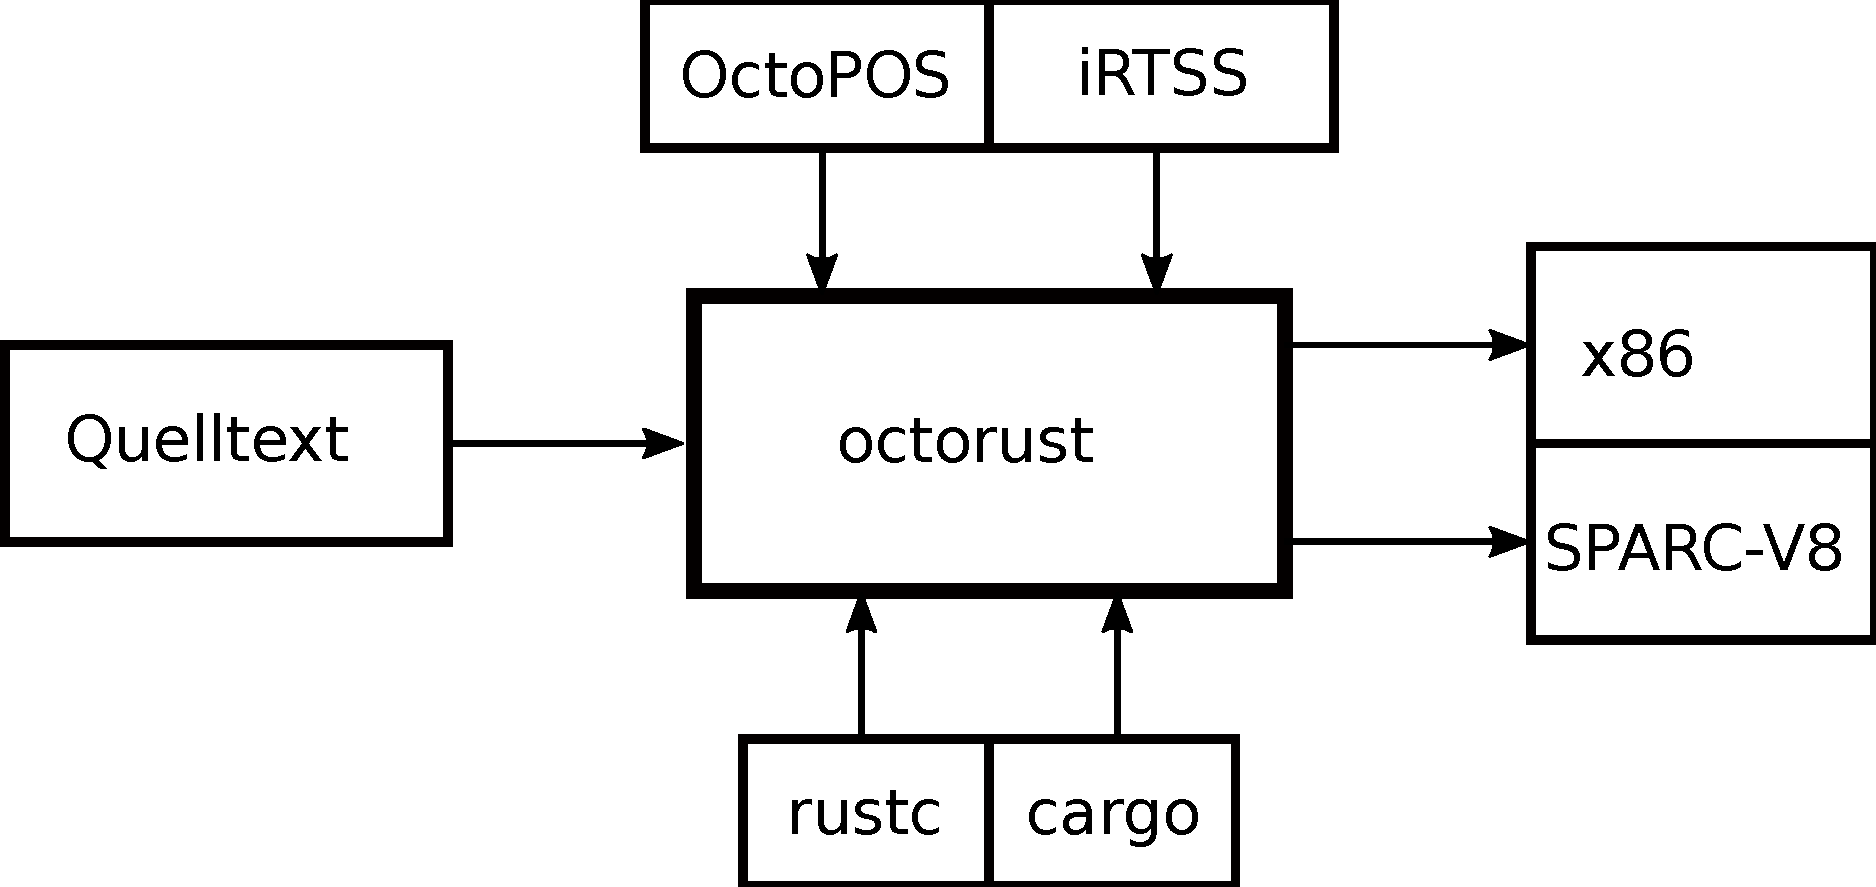
\includegraphics[width=0.6\textwidth]{images/octorust.pdf}
  \end{center}

\end{frame}

\begin{frame}{octolib}
    \begin{itemize}
      \item Rust-Bibliothek mit invasiven Strukturen und Funktionen
      \item Direkte C-Rust Bindings
      \item Rust-spezifische Anpassungen
        \begin{itemize}
          \item Objektorientierte Constraints
          \item Verwendung von Closures
          \item AgentClaim-Struktur
        \end{itemize}
      \item ca. 750 Zeilen Code (Rust)
    \end{itemize}
\end{frame}

%\lstdefinestyle{base}{
  language=C,
  emptylines=100,
  breaklines=true,
  basicstyle=\ttfamily\color{black},
  moredelim=**[is][\color{darkgreen}]{@}{@},
}


\lstset{showstringspaces=true,columns=fullflexible,keepspaces=true}

\begin{frame}[fragile]{Rust Bindings zur OctoPOS/iRTSS C-Schnittstelle}

  \begin{lstlisting}[frame=single,style=base]
    uint32_t get_value(void *data)
  \end{lstlisting}

  \begin{onlyenv}<1> {
    \begin{lstlisting}[frame=single,style=base]
      @extern crate libc;@
      @use libc::c_void;@




    \end{lstlisting}
  }
  \end{onlyenv}

  \begin{onlyenv}<2> {
    \begin{lstlisting}[frame=single,style=base]
      extern crate libc;
      use libc::c_void;

      @extern "C" {

      }@
    \end{lstlisting}
  }
  \end{onlyenv}

  \begin{onlyenv}<3> {
    \begin{lstlisting}[frame=single,style=base]
      extern crate libc;
      use libc::c_void;

      extern "C" {
        @fn get_value(data: *mut c_void) -> u32;@
      }
    \end{lstlisting}
  }
  \end{onlyenv}

\end{frame}
\lstdefinestyle{base}{
  language=C,
  emptylines=100,
  breaklines=true,
  basicstyle=\ttfamily\color{black},
  moredelim=**[is][\color{darkgreen}]{@}{@},
}


\lstset{showstringspaces=true,columns=fullflexible,keepspaces=true}

\begin{frame}[fragile]{Beispiel eines invasiven Rust-Programms}

  \begin{onlyenv}<1> {
    \begin{lstlisting}[frame=single,style=base]
      pub extern "C" fn rust_main_ilet (tile_id: u8) { // TODO Check tile_id name
        @//Invade
        let constraints = Constraints::new(4, 8);
        let claim = AgentClaim::new(constraints);@

        //Infect
        let ilet_fn = |param: *mut c_void| {
            print("Hello World!\n\0");
        }
        claim.infect(ilet_fn, None);

      } // Retreat & Shutdown
    \end{lstlisting}
  }
  \end{onlyenv}

\end{frame}
\begin{frame}{Evaluation}
    \begin{itemize}
      \item Rust wird mit C und X10 verglichen
      \item Wiederholte Laufzeitmessungen
      \item Betrachtung von Programmen mit und ohne Compiler-Optimierungen
    \end{itemize}
\end{frame}

\begin{frame}{Kompilierungsdauer}
  \begin{center}
    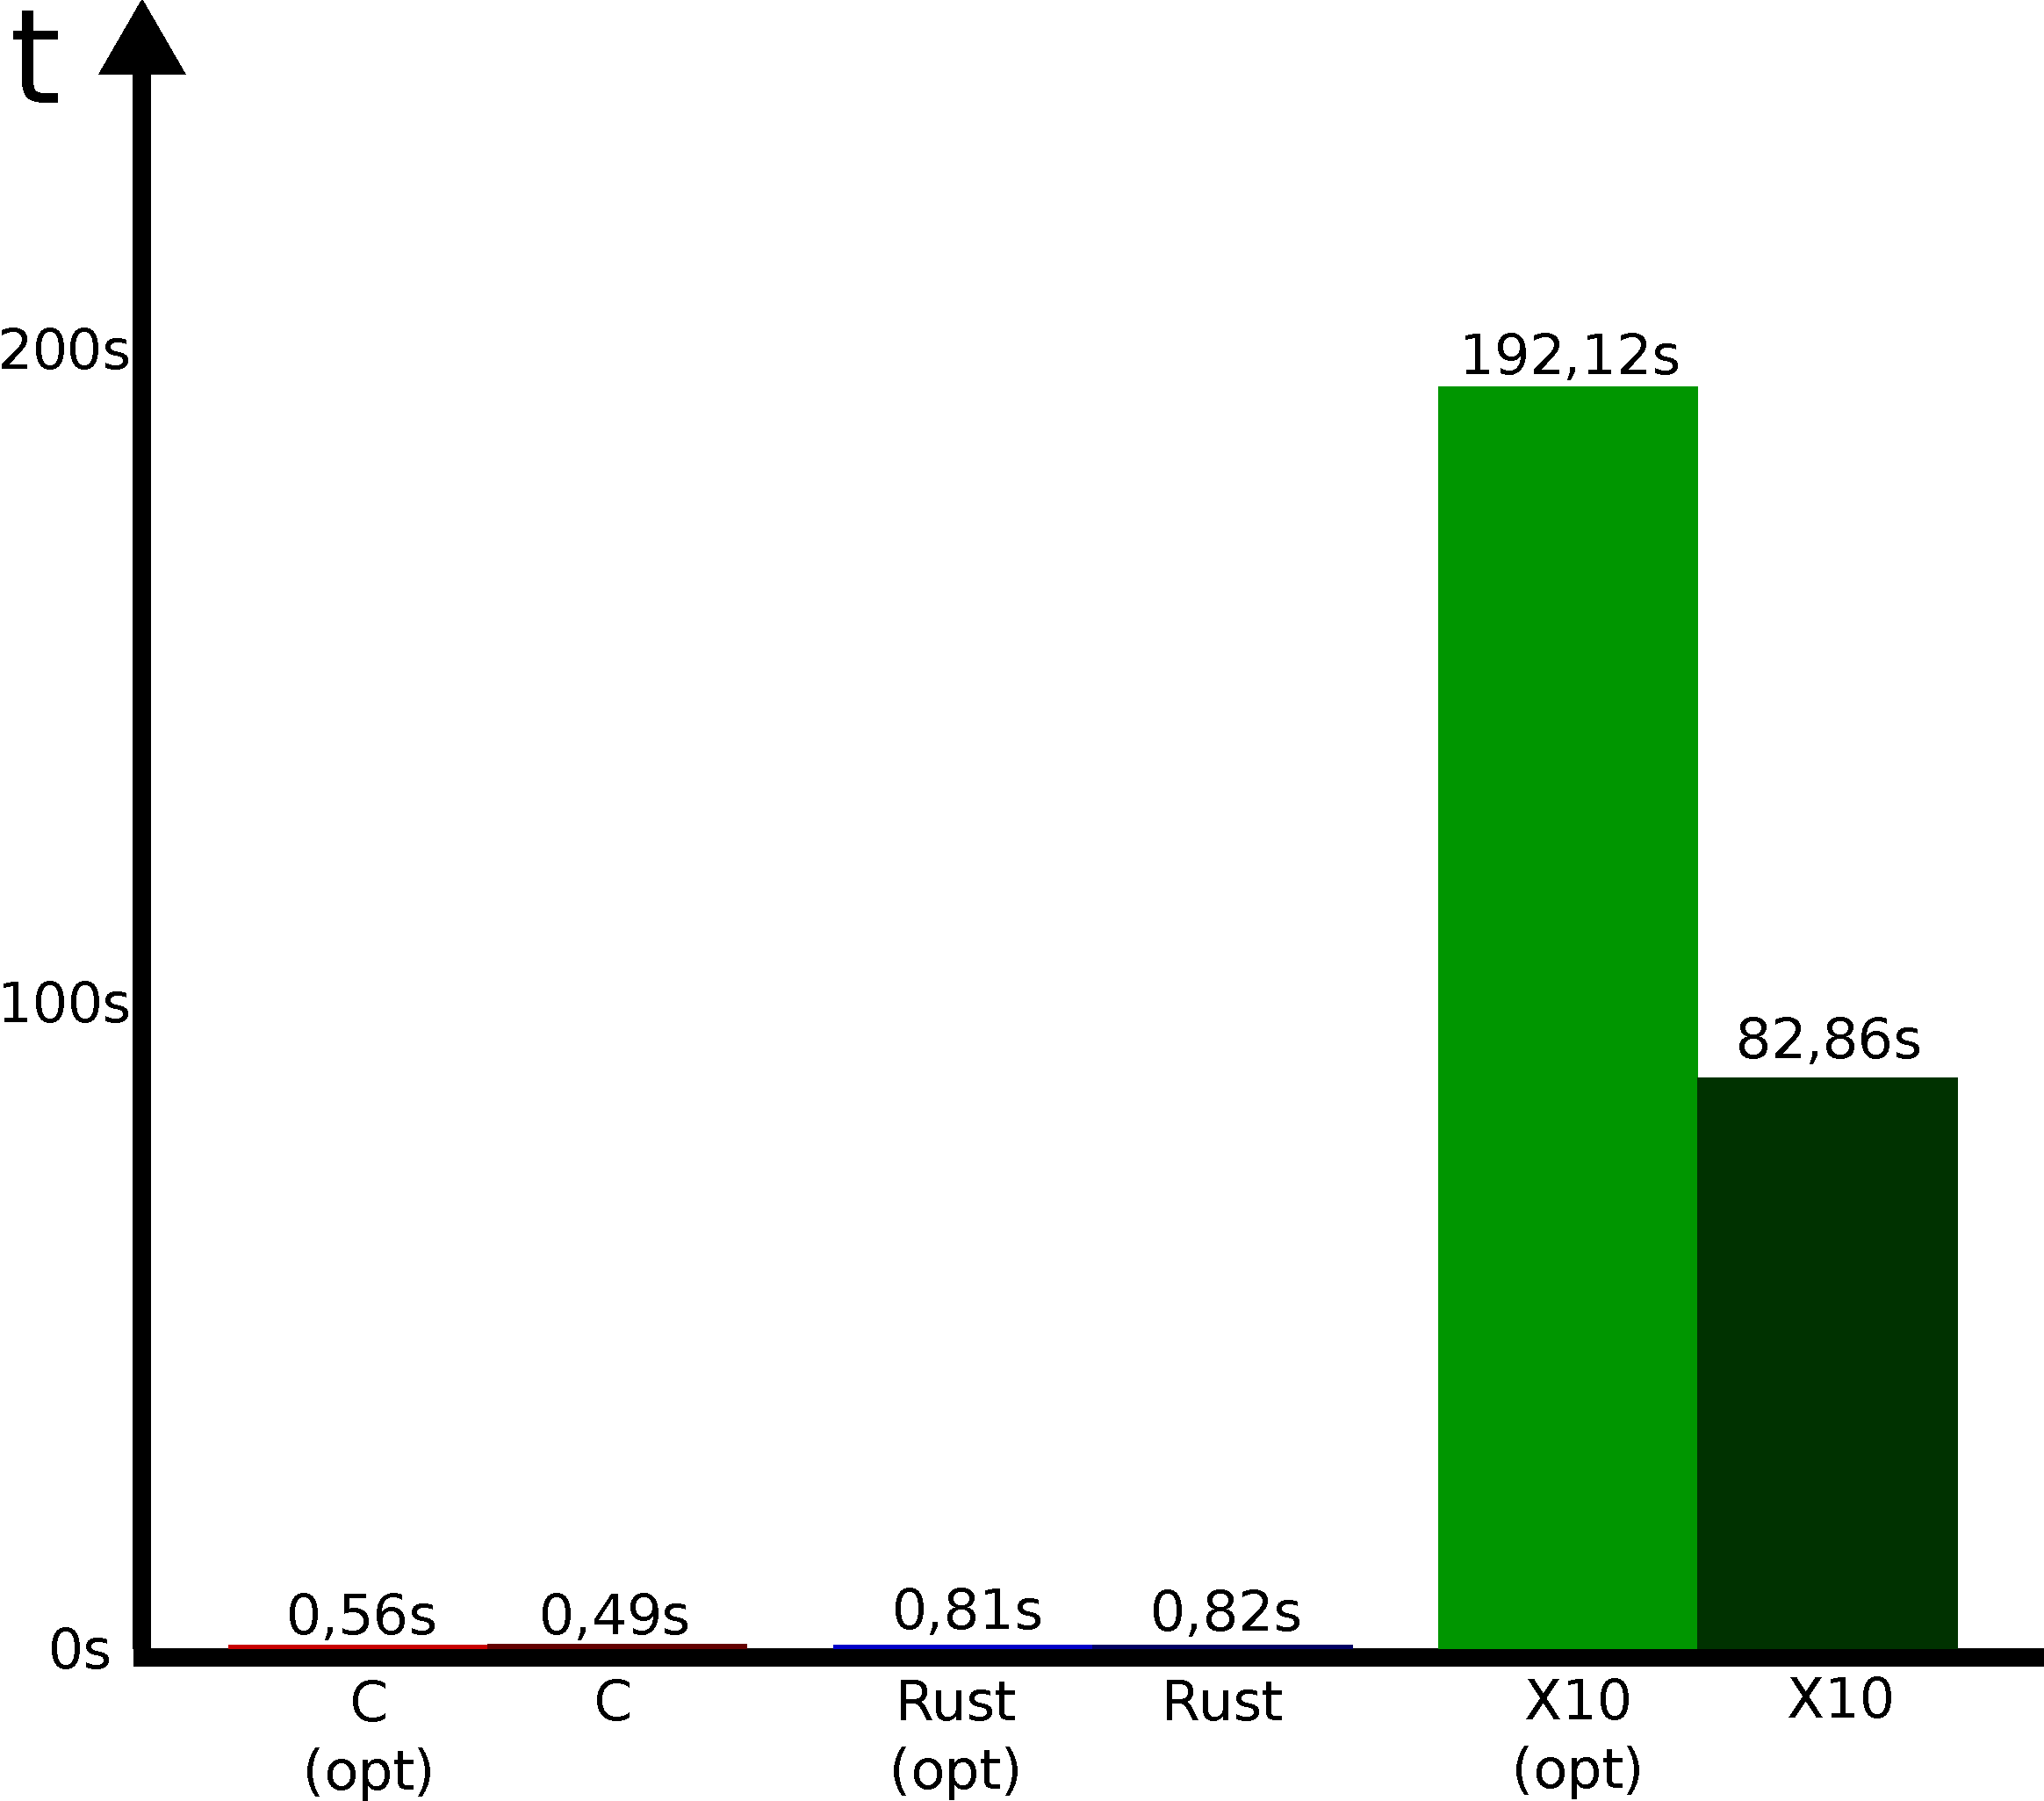
\includegraphics[width=0.55\textwidth]{images/compile-eval.pdf}
  \end{center}
  \begin{itemize}
    \item Zeitersparnis beim Kompilieren von Rust-Programmen im Vergleich mit X10-Programmen
  \end{itemize}
\end{frame}

\begin{frame}{Anlaufzeit}
  \begin{center}
    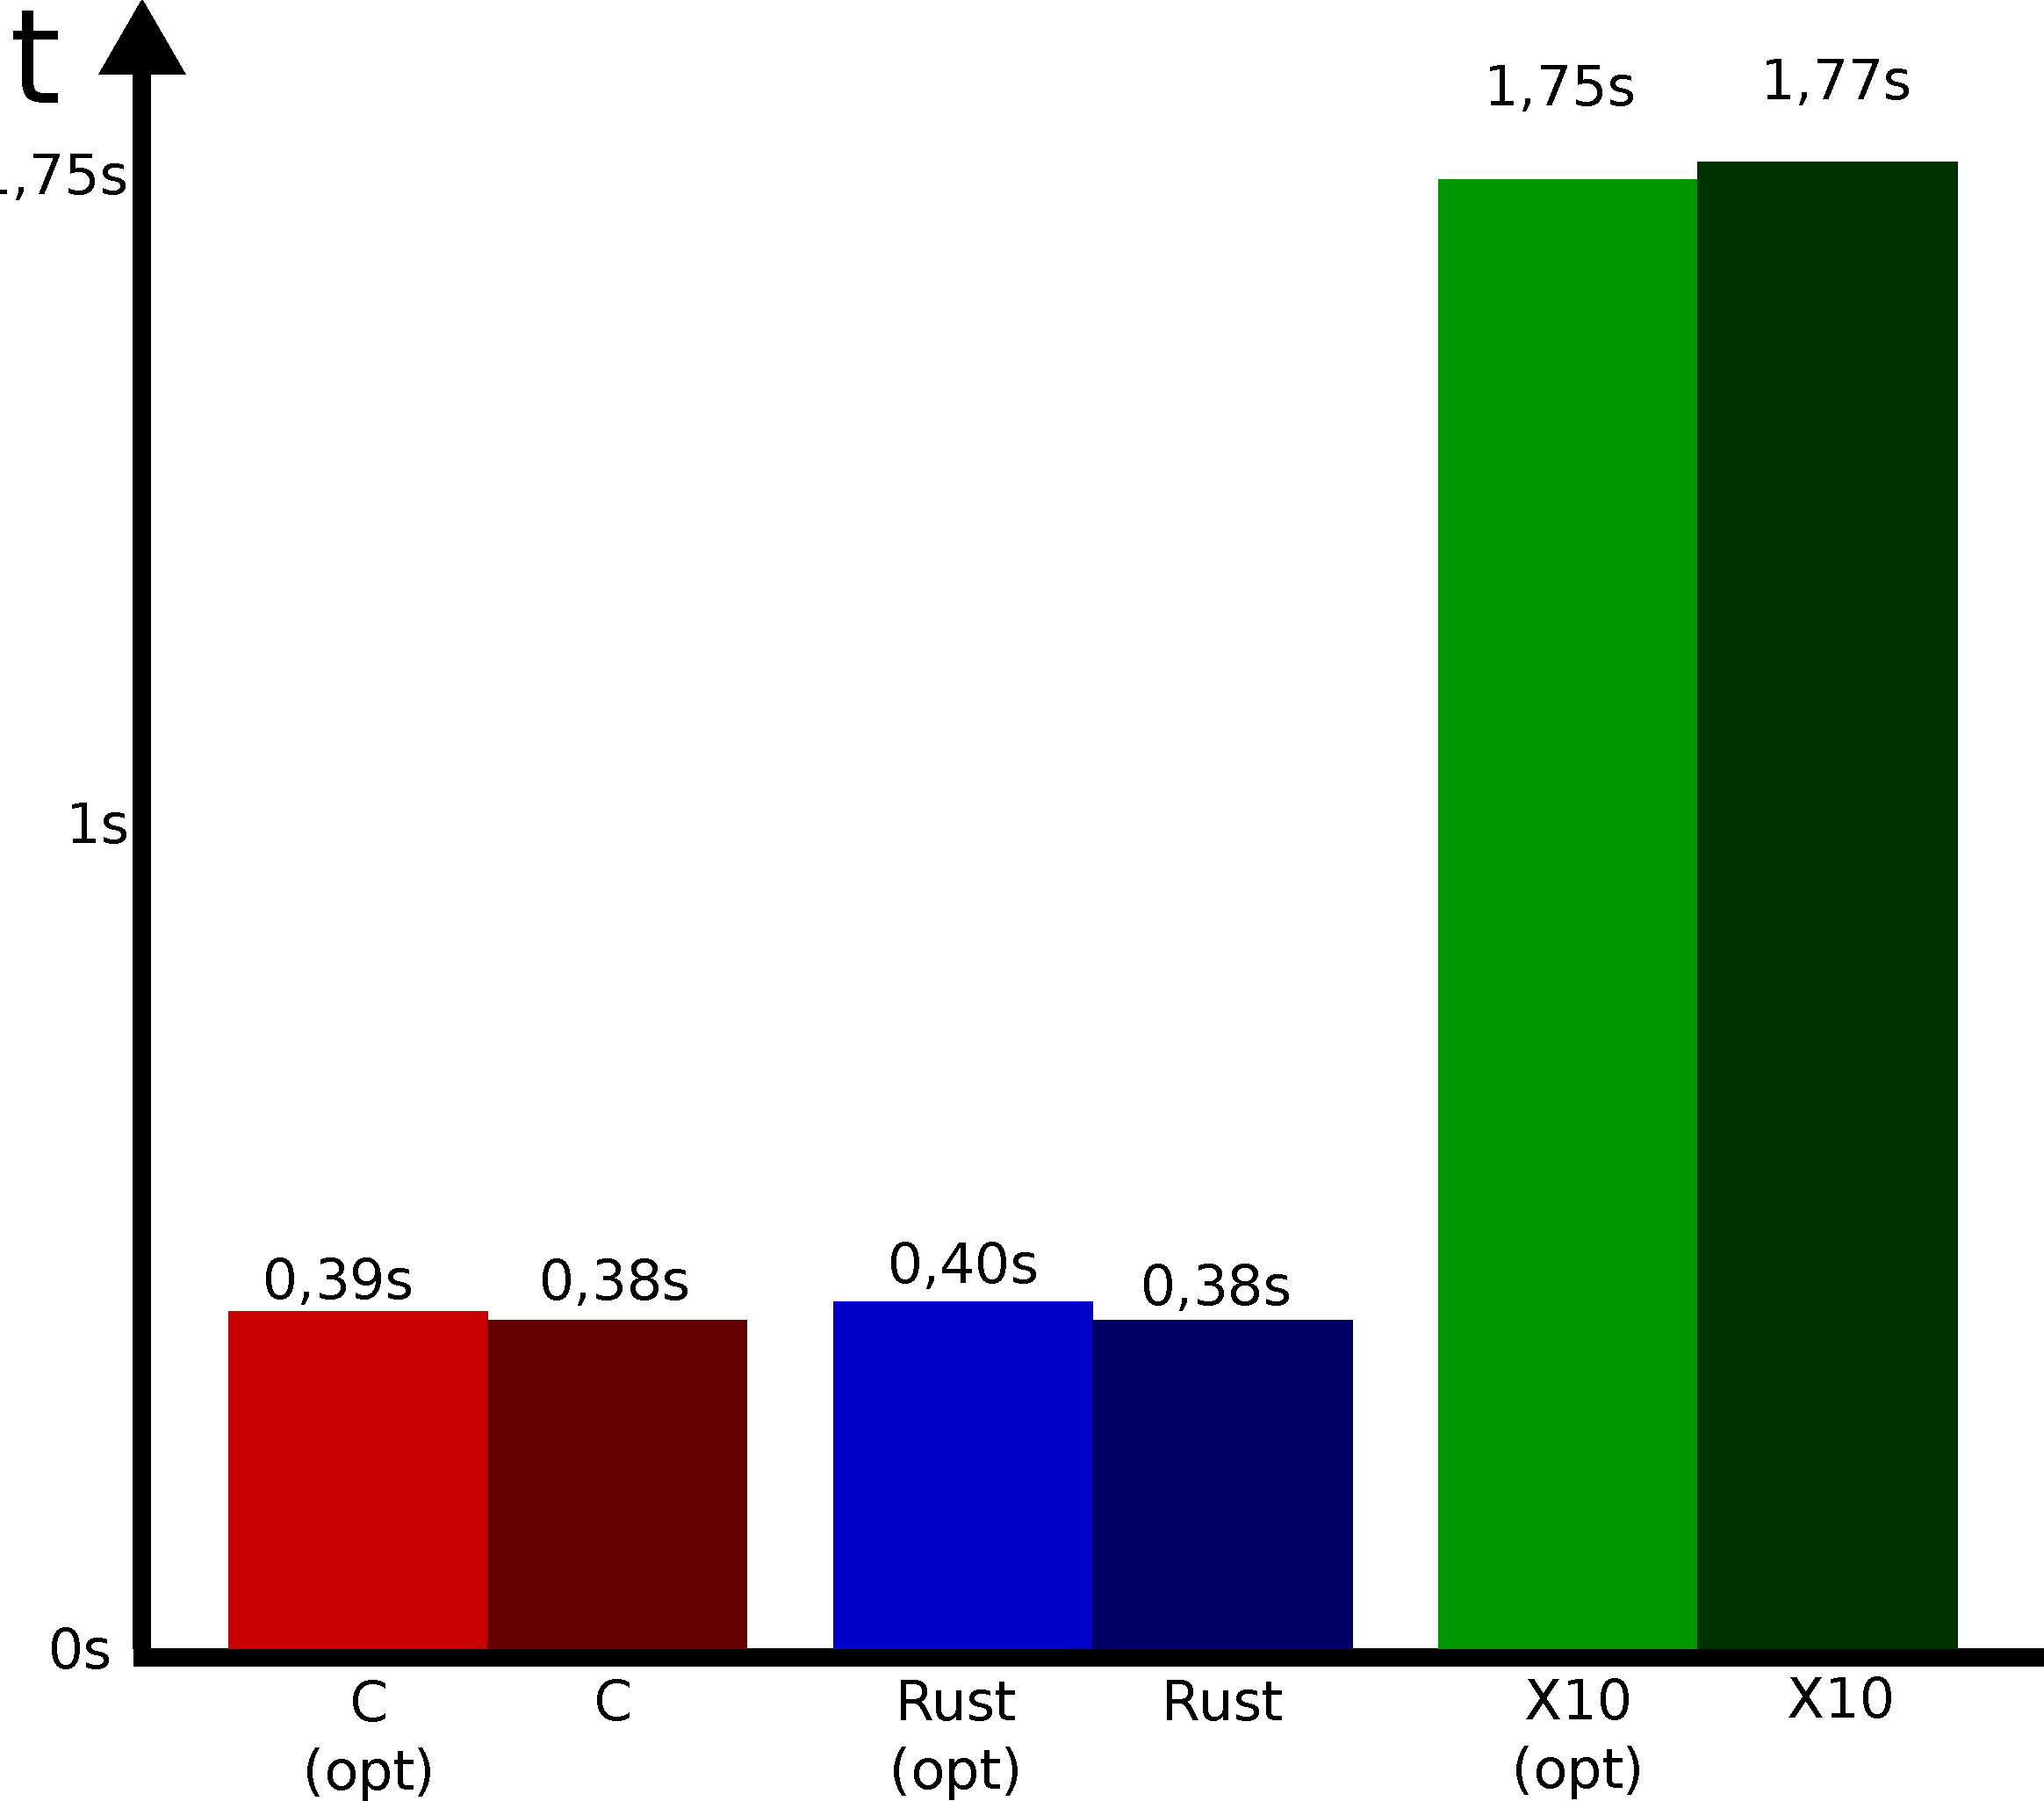
\includegraphics[width=0.55\textwidth]{images/startup-eval.pdf}
  \end{center}
  \begin{itemize}
    \item Rust und C benötigen ca. 1.4 Sekunden weniger um zu starten
  \end{itemize}
\end{frame}

\begin{frame}{Parallele Primzahlenberechnung}
  \begin{center}
    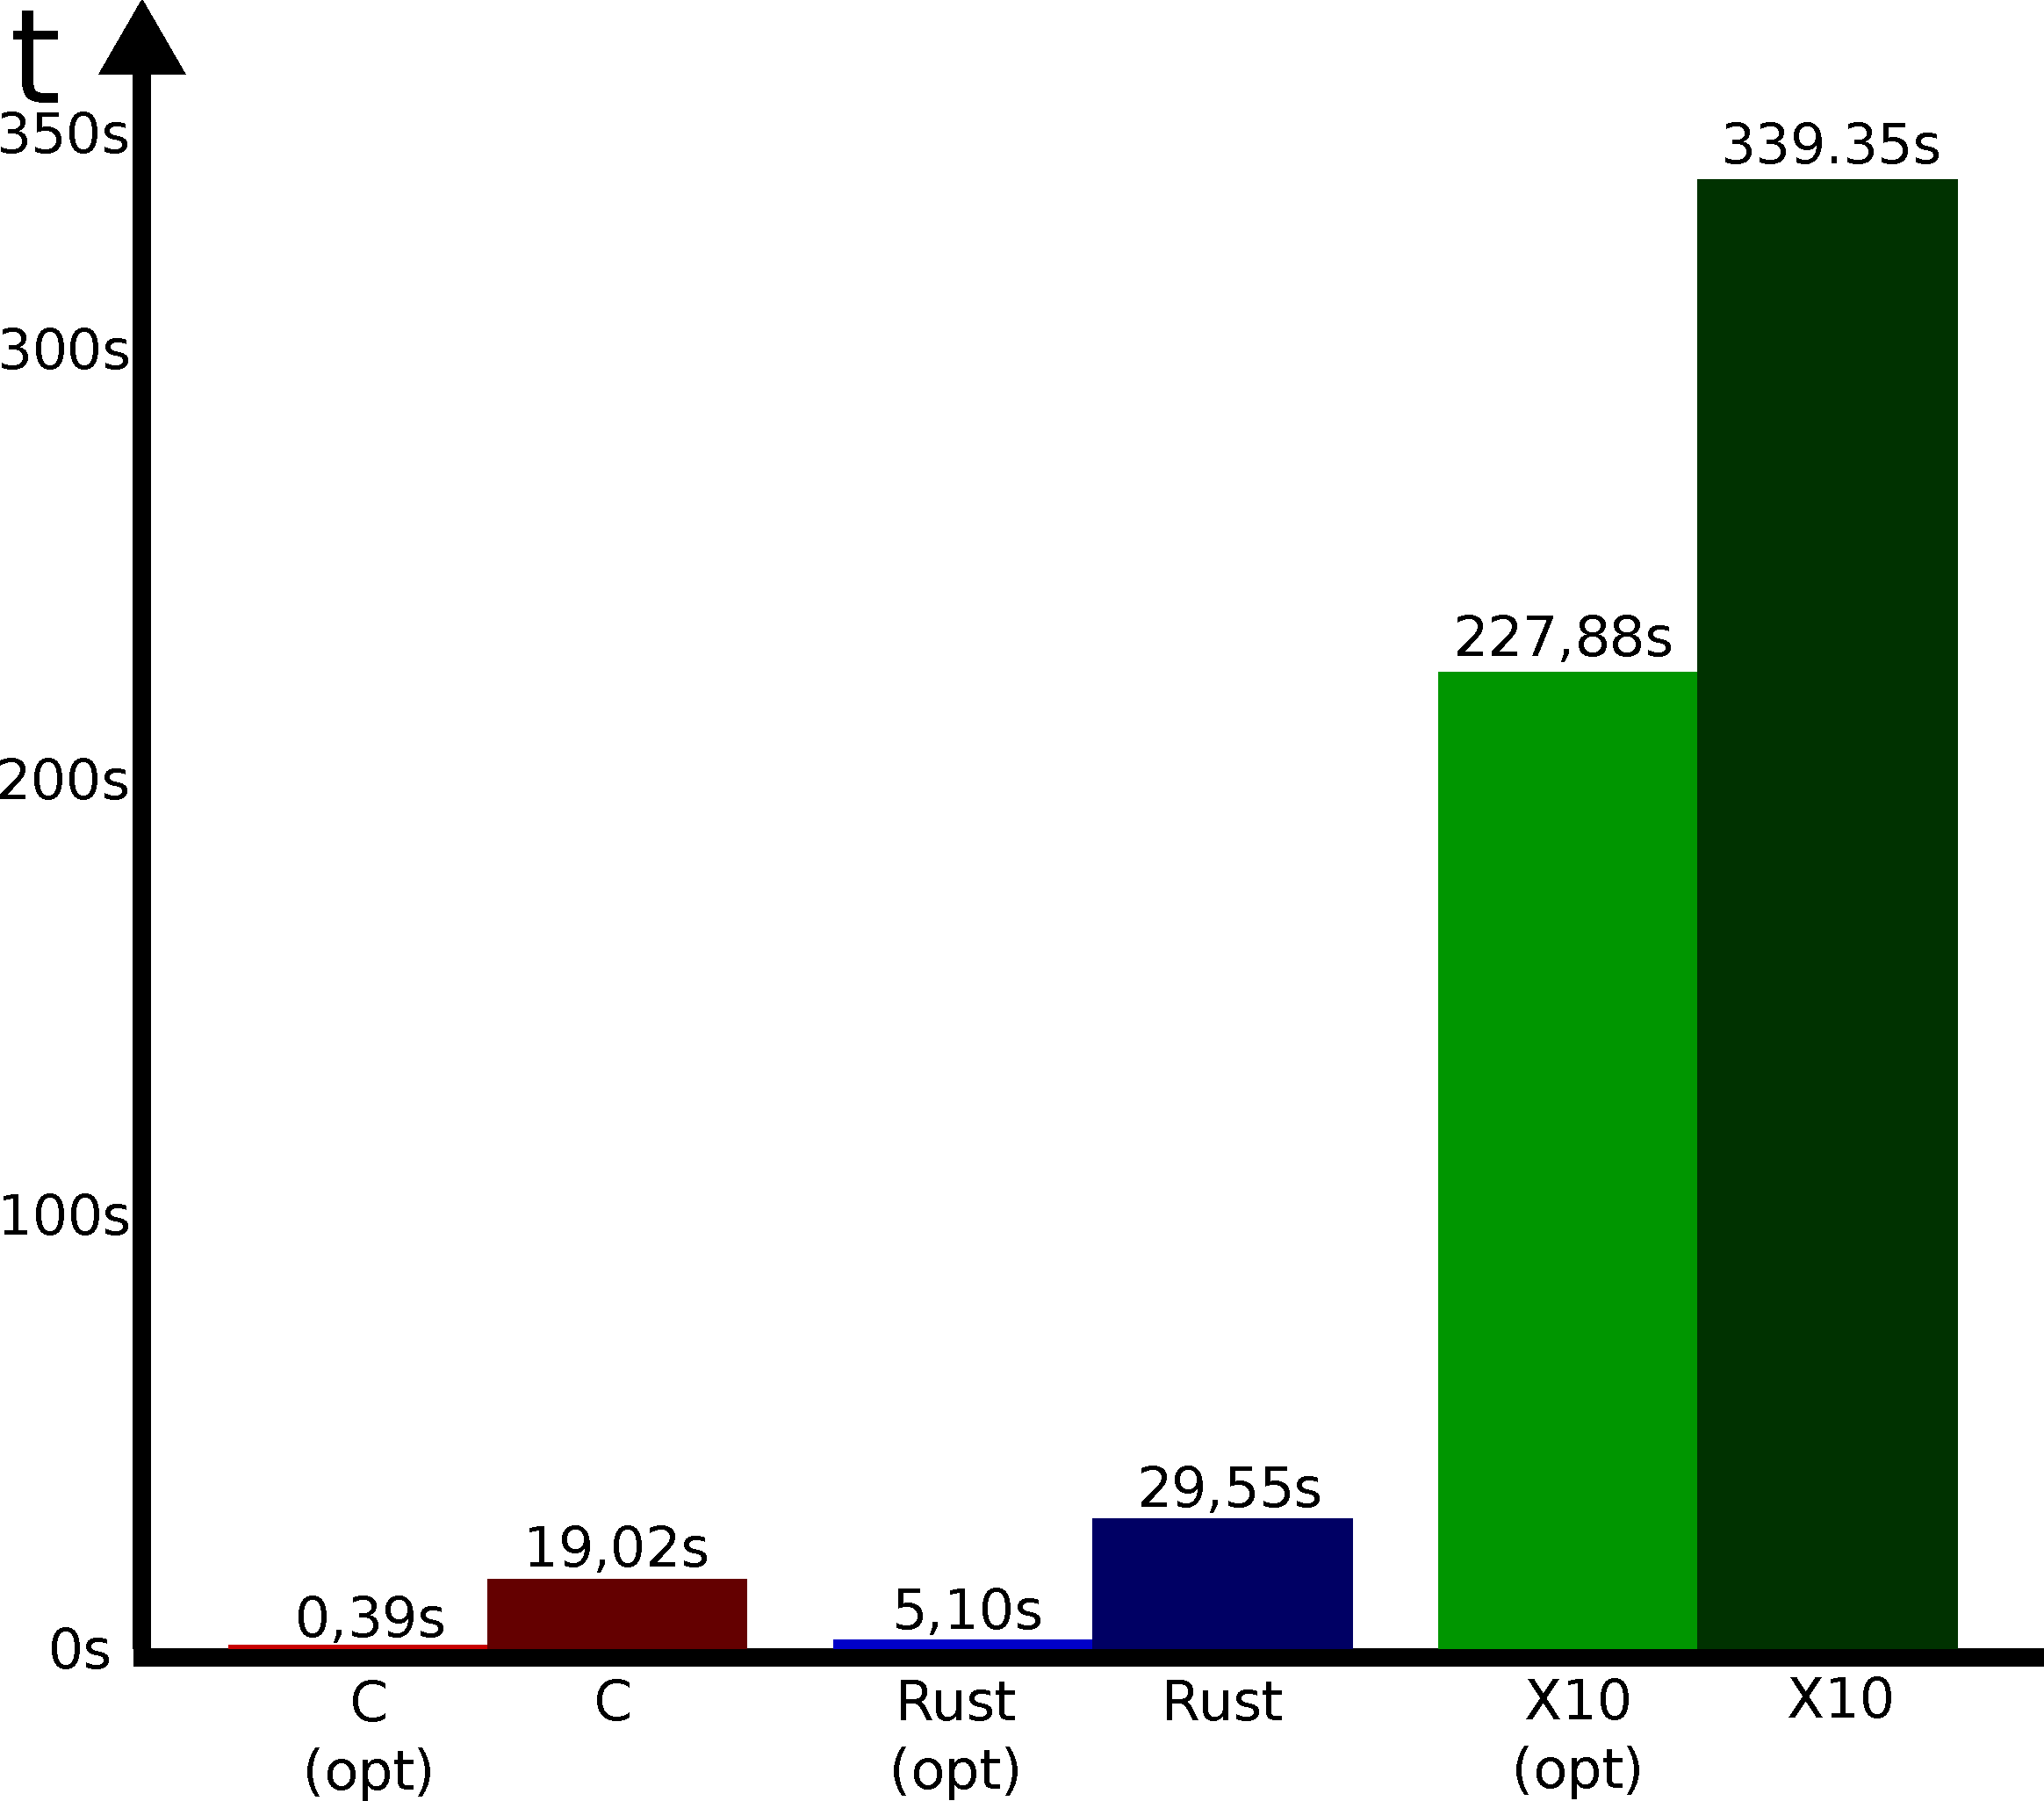
\includegraphics[width=0.55\textwidth]{images/primes-eval.pdf}
  \end{center}
  \begin{itemize}
    \item Rust weist bei Berechnung von Primzahlen keine Leistungsvorteile auf
  \end{itemize}
\end{frame}

\begin{frame}{Allokation von Objekten}
  \begin{center}
    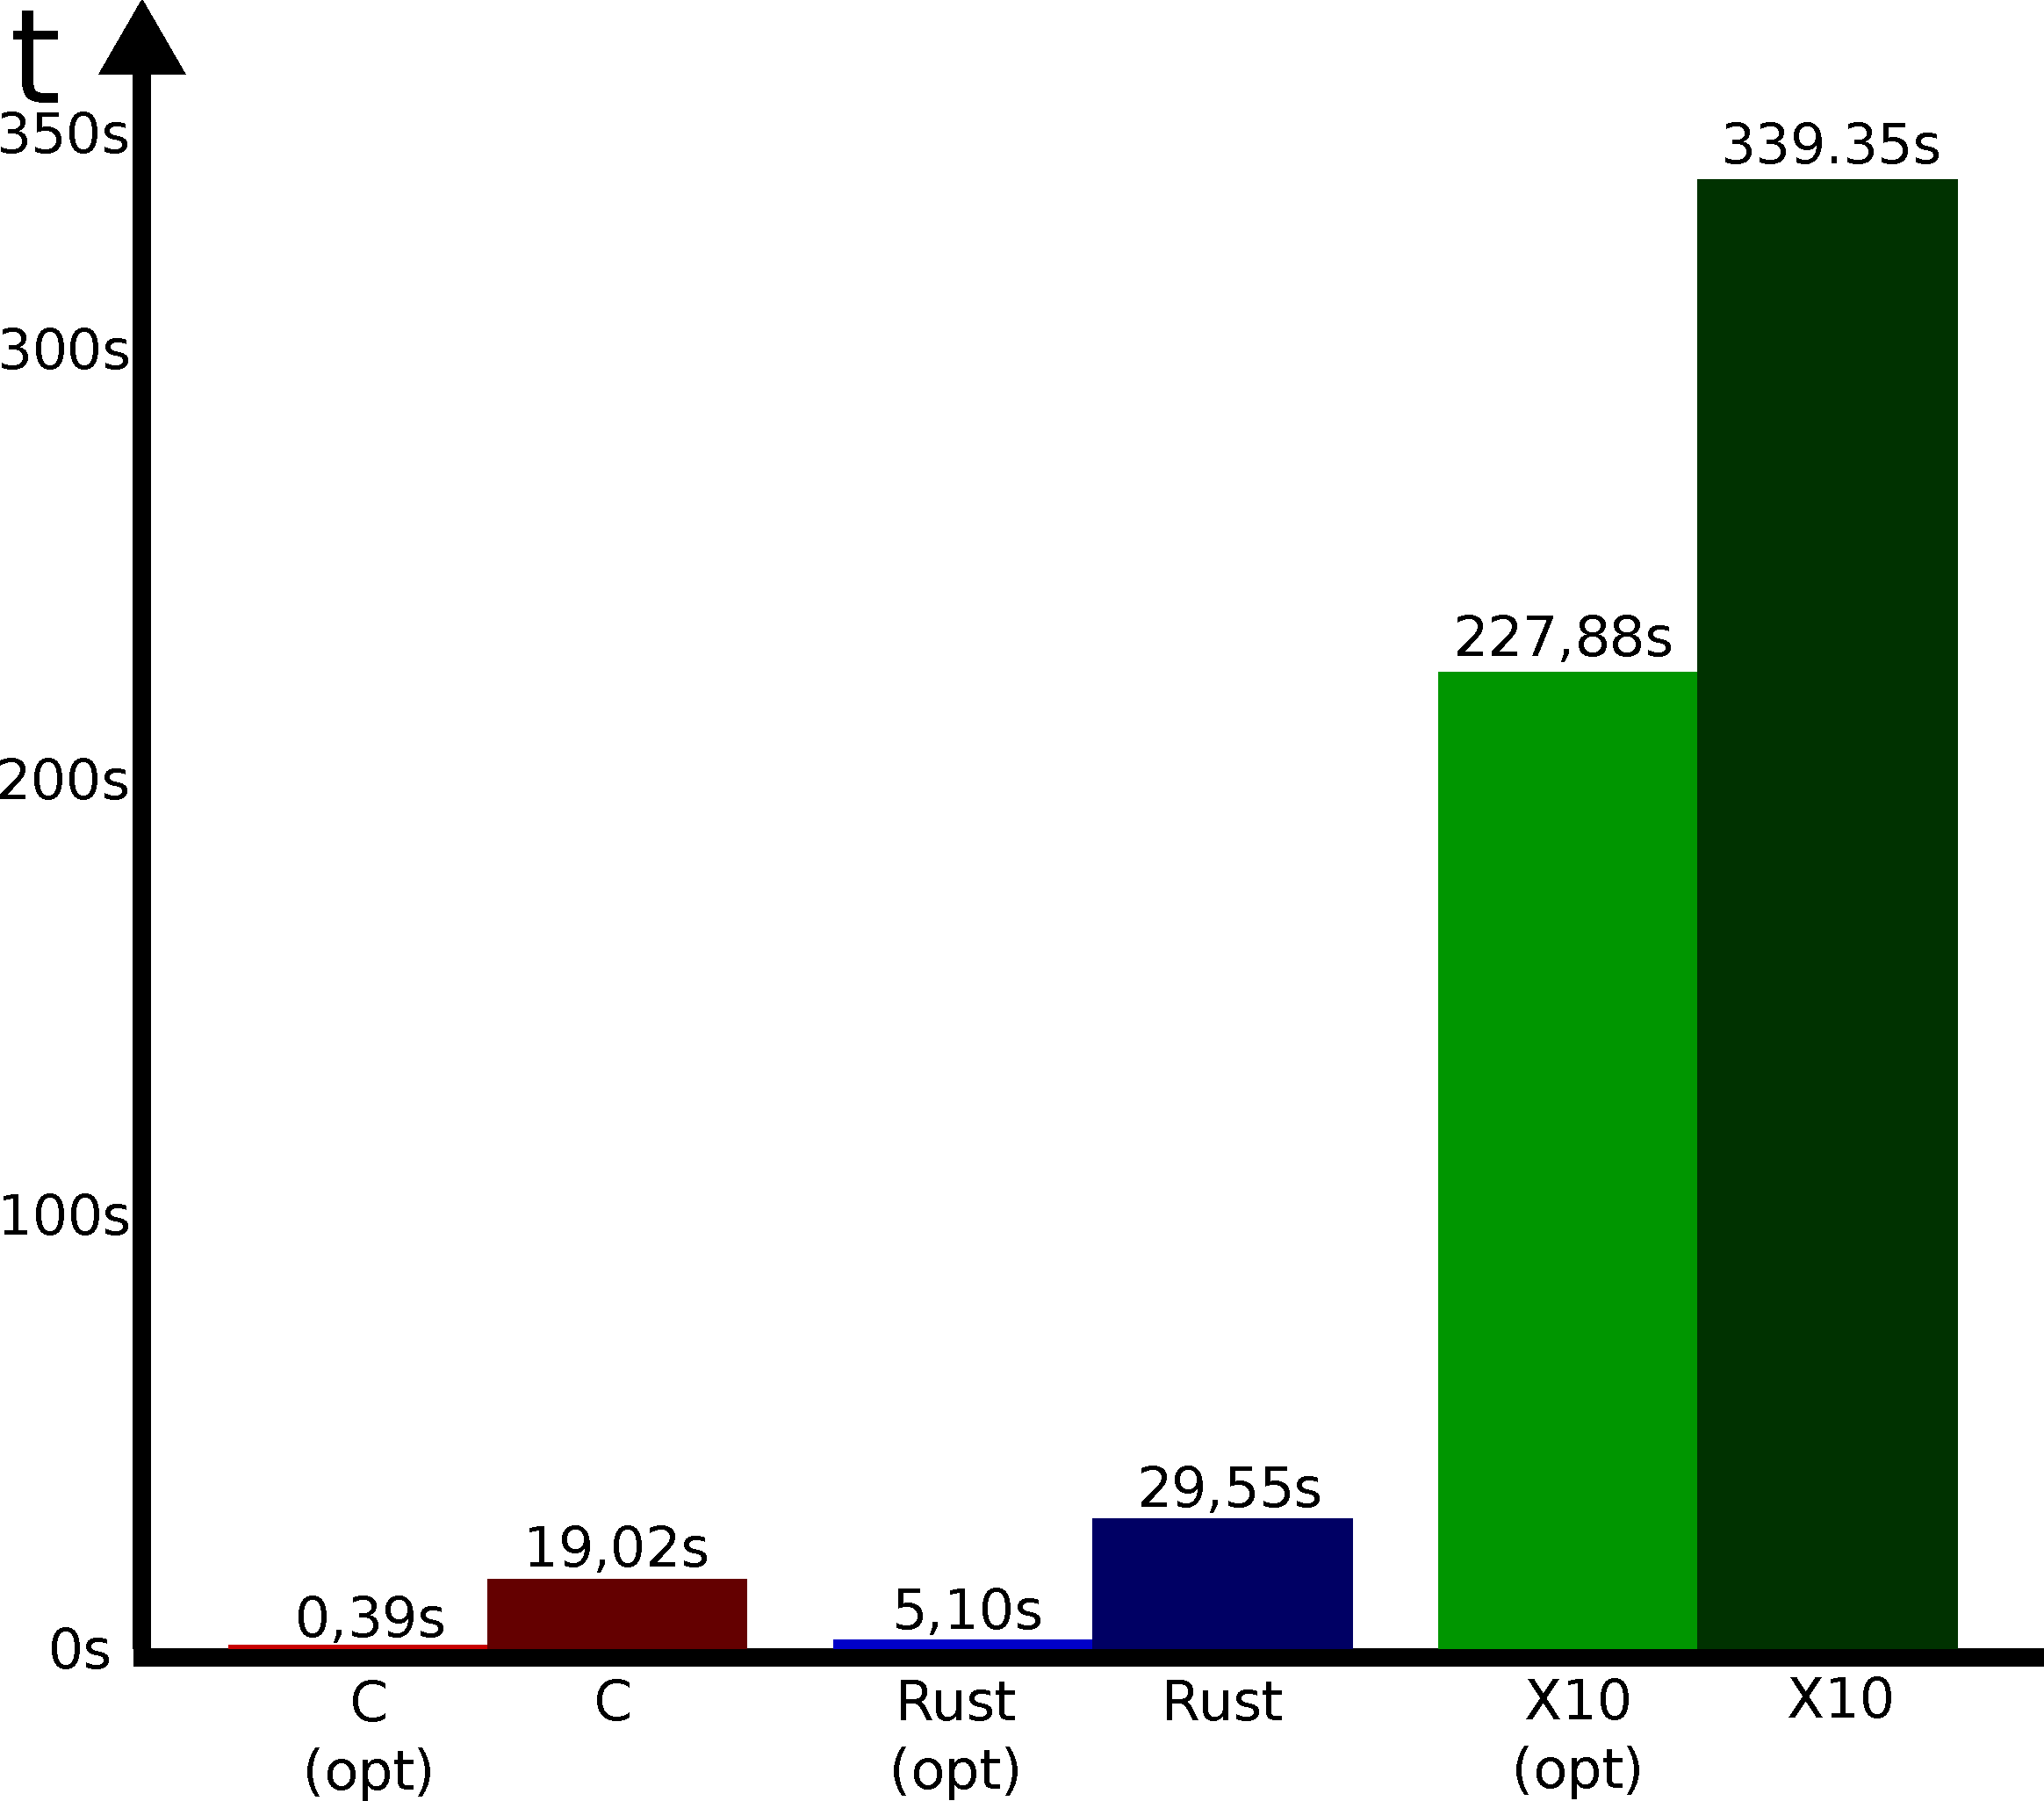
\includegraphics[width=0.55\textwidth]{images/garbage-eval.pdf}
  \end{center}
  \begin{itemize}
    \item C und Rust weisen eine mindestens 10-fach bessere Laufzeit als X10 auf
  \end{itemize}
\end{frame}


\begin{frame}{Zusammenfassung und Fazit}

  \begin{itemize}
    \item Invasives Rechnen ermöglicht ressourcenbewusstes Parallelrechnen
    \item Rust bietet Speichersicherheit ohne Garbage Collector
    \item Rust schützt vor undefinertem Verhalten
    \item octorust und octolib ermöglichen den Einsatz von Rust im invasiven Rechnen
    \item Rust weist in speicherintensiven Szenarien bessere Laufzeiten als X10 auf
  \end{itemize}

\end{frame}

\begin{frame}{Vielen Dank für ihre Aufmerksamkeit}
  \begin{columns}[t]
    % convert -density 150 present.pdf -quality 90 build/output.png
    % Befehl vor make ausführen
    \column{.1\textwidth}

    \column{.4\textwidth}
      \centering
      \includegraphics[width=5cm,height=3.5cm]{build/output-6.png}
      \includegraphics[width=5cm,height=3.5cm]{build/output-48.png}

    \column{.4\textwidth}
      \centering
      \includegraphics[width=5cm,height=3.5cm]{build/output-10.png}
      \includegraphics[width=5cm,height=3.5cm]{build/output-55.png}

    \column{.1\textwidth}
  \end{columns}
\end{frame}

\end{document}

% {
% Roten Faden
% AgentClaim etc zum ersten Beispiel zurückführen
% Rust Invasiv Code Beispiel
% }

% Affine Typen

% Erstes Rust Beispiel raus

% Dependent types (Kann als Frage vorkommen) -X10 het's, Rust nicth, was verliert man dadurch?
% In X10 nur halbherzig implementiert, werden kaum benutzt
% RFC 200 Rust

% 15:45 Montag, 13. November
